\documentclass[a4paper]{book}
\usepackage[T1]{fontenc}

\usepackage[utf8]{inputenc}
\usepackage[margin=2cm]{geometry}
\geometry{verbose}
\pagestyle{plain}
\setcounter{secnumdepth}{6}
\setcounter{tocdepth}{2}
\usepackage[usenames,dvipsnames]{xcolor}
\usepackage{graphicx}
\usepackage{tikz}
\usetikzlibrary{positioning,shapes,shadows,arrows,matrix,fit,calc}
\usepackage{array}
\usepackage{textcomp}
\usepackage{amssymb}
\usepackage{adjustbox}
\usepackage{enumitem}
\usepackage[unicode=true,
 bookmarks=false,
 breaklinks=false,pdfborder={0 0 1},backref=section,colorlinks=false]
 {hyperref}
\hypersetup{colorlinks,linkcolor={red!50!black},citecolor={blue!50!black},urlcolor={blue!80!black}}

\usepackage{fixltx2e}
\usetikzlibrary{mindmap}
\pgfdeclarelayer{background}
\pgfdeclarelayer{foreground}
\pgfdeclarelayer{}
\pgfsetlayers{background,main,foreground}

%%%%%%%%%%%%%%%%%%%%%%%%%%%%%% LyX specific LaTeX commands.
%% Because html converters don't know tabularnewline
\providecommand{\tabularnewline}{\\}

%%%%%%%%%%%%%%%%%%%%%%%%%%%%%% User specified LaTeX commands.
%&pdfLaTeX
% !TEX encoding = UTF-8 Unicode
\usepackage{ifxetex}
\ifxetex
\usepackage{fontspec}
\else
\fi
\usepackage{titlesec}
\usepackage{textcomp}
\usepackage{array}
\usepackage{ulem}
\usepackage{mdwlist}
\usepackage{fancyhdr}
\usepackage{lastpage}
\fancypagestyle{plain}{
	\fancyhf{}% Clear header/footer
	%\fancyhead[R]{\includegraphics[width=3cm]{images/ACTETDHeader.png}}
	\fancyhead[L]{\textit{{Solution Architecture Description}}}
	\fancyfoot[L]{\textit{{Edition 0P1: Version 202205101500}}}
	\fancyfoot[C]{\textit{{\today}}}
	\fancyfoot[R]{\textit{{\thepage/\pageref{LastPage}}}}
}
\pagestyle{plain}
\renewcommand{\headrulewidth}{1pt}
\renewcommand{\footrulewidth}{1pt}

\usepackage{titlesec}
\usepackage{parskip}
\usepackage{tabu}
\usepackage{multirow}

\usepackage[xindy, toc]{glossaries}

\parskip=6pt

\titlespacing*{\section}{0pt}{1ex}{0.5ex}
\titlespacing*{\subsection}{0pt}{1ex}{0.5ex}
\titlespacing*{\subsubsection}{0pt}{1ex}{0.5ex}

\titleformat{\paragraph}[hang]{\normalfont\normalsize\bfseries}{\theparagraph}{1em}{}
\titlespacing*{\paragraph}{0pt}{1ex}{0.5ex}

\titleformat{\subparagraph}[hang]{\normalfont\normalsize\bfseries}{\thesubparagraph}{1em}{}
\titlespacing*{\subparagraph}{0pt}{1ex}{0.5ex}

\color{black}

\usepackage{chngcntr}
\counterwithin*{chapter}{part}
\makeatother

\makeglossary

\newcommand{\cmcapability}[1 ]{\textsc{\textcolor{OliveGreen}{#1}}}
\newcommand{\cmdelivery}[1 ]{{\textsc{\textcolor{Violet}{#1}}}}
\newcommand{\cmservice}[1 ]{\textit{\textcolor{OliveGreen}{#1}}}

\newcommand{\dricats}{\textsc{\textcolor{Purple}{\small{DRICaTS }}}}
\newcommand{\dricatsrelease}{\textcolor{Purple}{2.0.0}}
\newcommand{\petasos}{\textsc{\textcolor{Purple}{\small{Petasos }}}}

\newcommand{\ponos}{\textsc{\textcolor{Purple}{\small{Ponos }}}}
\newcommand{\ponosim}{\textsc{\textcolor{Purple}{\small{Ponos-IM }}}}
\newcommand{\ponosdm}{\textsc{\textcolor{Purple}{\small{Ponos-DM }}}}
\newcommand{\ponospm}{\textsc{\textcolor{Purple}{\small{Ponos-PM }}}}
\newcommand{\ponosdb}{\textsc{\textcolor{Purple}{\small{Ponos-DB }}}}

\newcommand{\dricatsnavigator}{\textsc{\textcolor{Purple}{\small{DRICaTS-Navigator }}}}

\newcommand{\HRule}{\rule{0.8\linewidth}{0.5mm}}

\newcommand{\fhirtask}{\textsc{\textcolor{Blue}{\small{FHIR::Task }}}}
\newcommand{\fhirprovenance}{\textsc{\textcolor{Blue}{\small{FHIR::Provenance }}}}
\newcommand{\fhirlocation}{\textsc{\textcolor{Blue}{\small{FHIR::Location }}}}
\newcommand{\fhirpatient}{\textsc{\textcolor{Blue}{\small{FHIR::Patient }}}}
\newcommand{\fhirpractitioner}{\textsc{\textcolor{Blue}{\small{FHIR::Practitioner }}}}

\newcommand{\jgroups}{\textit{\textcolor{gray}JGroups }}

\newcommand{\postgres}{\textit{\textcolor{gray}Postgres }}
\newcommand{\postgresversion}{\textit{\textcolor{gray}to be defined!}}

\newcommand{\wildfly}{\textit{\textcolor{gray}Wildfly }}
\newcommand{\wildflyversion}{\textit{\textcolor{gray}24.01 }}


\begin{document}
\begin{titlepage}
	\begin{center}

		%\includegraphics[width=5cm]{images/ACTETDMain.png}~\\[1cm]

			% Title
		\HRule \\[0.4cm]
		{ \huge \bfseries DRICATS-Health Solution Architecture\\[0.4cm] }
		Distributed/Resilient Integration, Collaboration and Tasking Services \\
		for Health Information Systems

		\HRule \\[1.5cm]


		\vfill

		% Bottom of the page
		{\large \today}

	\end{center}
\end{titlepage}

\tableofcontents

\part{DRICATS - An Overview}

\chapter{Strategy}

\chapter{Implementation}

\section{Open Source Frameworks}

The following \textit{Open Source} software packages within the DRICATS solution.

\begin{itemize}
 \item Infinispan\textsuperscript{\textregistered}:
"Infinispan and the Infinispan logo are trademarks of Red Hat, Inc."
 \item Wildfly\textsuperscript{\textregistered}:
"Wildfly and the Wildfly logo are trademarks of Red Hat, Inc."
\end{itemize}


\part{Business Architecture}

\part{Information Systems Architecture}
\chapter{Information Architecture}

\chapter{Application Architecture}
\section{Overview}

\begin{figure}[h!]
	\begin{adjustbox}{max size={0.98\textwidth}{0.9\textheight}, center}
		\includegraphics[]{diagrams/DRICATS-DesignOverview.png}
	\end{adjustbox}
	\caption{DRICATS Solution Architecture - High Level}
\end{figure}

\section{Integration Modules}

\section{DigitalTwin / Workflow}

\section{Core}
\subsection{Ponos (Task Assurance / Reporting)}
\subsubsection{Overview}

\ponos is the \textit{Task Assurance} engine of \dricats for \textbf{internal} tasks (i.e. message processing, workflows, etc.). It provides the resilience and recovery services for \textit{Tasks} and ensures \textit{Tasks} are completed within a well-defined period or suitable retry and/or failure reporting actions are instigated.

It is important to reiterate that \ponos manages \textbf{internal} \textit{Tasks}. It is \textbf{NOT} manage Tasking or Workflow activities for general practitioners within the clinical or administrative domains.

\begin{figure}[h!]
	\begin{adjustbox}{max size={0.98\textwidth}{0.9\textheight}, center}
        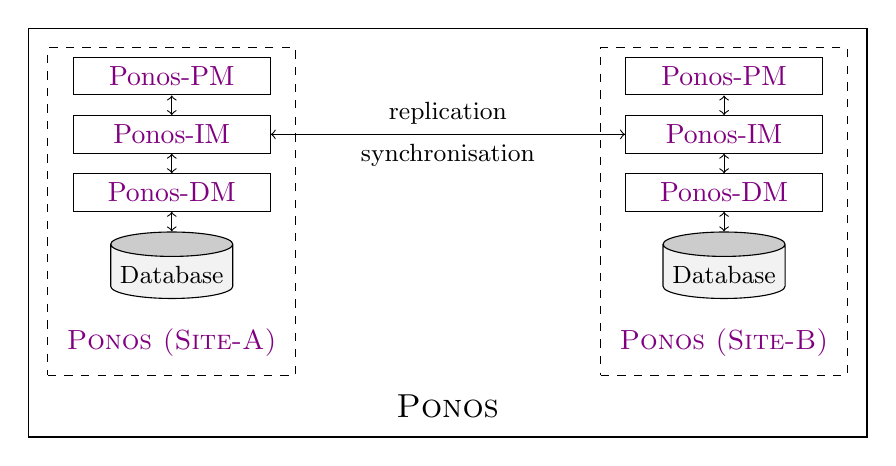
\begin{tikzpicture}[node distance=0.5cm]
            \node[draw,rectangle, minimum width = 2.5cm](ponospm-site-a){\color{Purple}Ponos-PM};
            \node[draw,rectangle, minimum width = 2.5cm, below=of ponospm-site-a, yshift=0.25cm](ponosim-site-a){\color{Purple}Ponos-IM};
            \draw[<->](ponospm-site-a.south)--(ponosim-site-a.north);
            \node[draw,rectangle, minimum width = 2.5cm, below=of ponosim-site-a, yshift=0.25cm](ponosdm-site-a){\color{Purple}Ponos-DM};
            \draw[<->](ponosim-site-a.south)--(ponosdm-site-a.north);
            \node[draw, cylinder, cylinder uses custom fill, cylinder body fill = gray!10, cylinder end fill = gray!40, aspect = 0.2, shape border rotate = 90, , below=of ponosdm-site-a, yshift=0.25cm](ponosdb-site-a){\small{Database}};
            \draw[<->](ponosdm-site-a.south)--(ponosdb-site-a.north);
            \node[rectangle, below=of ponosdb-site-a,yshift=0.25cm](ponoslabel-site-a){\color{Purple}\textsc{Ponos (Site-A)}};
            \node[draw,rectangle,dashed, fit=(ponospm-site-a) (ponoslabel-site-a)](ponos-site-a){};

            \node[draw,rectangle, minimum width = 2.5cm, right=of ponospm-site-a, xshift=4cm](ponospm-site-b){\color{Purple}Ponos-PM};
            \node[draw,rectangle, minimum width = 2.5cm, below=of ponospm-site-b, yshift=0.25cm](ponosim-site-b){\color{Purple}Ponos-IM};
            \draw[<->](ponospm-site-b.south)--(ponosim-site-b.north);
            \node[draw,rectangle, minimum width = 2.5cm, below=of ponosim-site-b, yshift=0.25cm](ponosdm-site-b){\color{Purple}Ponos-DM};
            \draw[<->](ponosim-site-b.south)--(ponosdm-site-b.north);
            \node[draw, cylinder, cylinder uses custom fill, cylinder body fill = gray!10, cylinder end fill = gray!40, aspect = 0.2, shape border rotate = 90, , below=of ponosdm-site-b, yshift=0.25cm](ponosdb-site-b){\small{Database}};
            \draw[<->](ponosdm-site-b.south)--(ponosdb-site-b.north);
            \node[rectangle, below=of ponosdb-site-b,yshift=0.25cm](ponoslabel-site-b){\color{Purple}\textsc{Ponos (Site-B)}};
            \node[draw,rectangle,dashed, fit=(ponospm-site-b) (ponoslabel-site-b)](ponos-site-b){};

            \draw[<->](ponosim-site-a.east)--(ponosim-site-b.west) node [above, midway]{\small{replication}} node [below, midway]{\small{synchronisation}};

            \node[rectangle, fit=(ponos-site-a) (ponos-site-b)](ponos-drawing){};
            \node[rectangle, below=of ponos-drawing, yshift=0.5cm](ponos-label){\textsc{\large{Ponos}}};
            \node[draw, rectangle, fit=(ponos-drawing) (ponos-label)](ponos-drawing){};
        \end{tikzpicture}
	\end{adjustbox}
	\caption{Ponos (Site-A + Site-B)}
	\label{fig:ponos-overview}
\end{figure}

The above diagram provides a (very) high level view of the \ponos architecture, illustrating a multi-site\footnote{Note that whilst the above diagram (Figure \ref{fig:ponos-overview}) illustrates a dual site scenario, the solution can be deployed with 1+n sites, where n > 0. In the circumstance where deployment is at a single site, some further consideration to resilience and recovery strategies may be required.} deployment architecture\footnote{Note also that where n > 1 (i.e. the number sites is 3 or more), the framework for resilience forms a mesh with no single ``site'' being a single point of failure.}.

\subsubsection{Ponos-PM}
\paragraph{Overview}

\ponospm is a web-based user interface implemented as part of the \dricatsnavigator module. It provides a \textit{User Interface} for the following activities:
\begin{enumerate}[noitemsep]
 \item \textit{Task Status Visualisation:} view a \textit{Task} detail - including all metadata and status information or both active and historical (finalised or failed) \textit{Tasks};
 \item \textit{Task Journey (Aggregate Task) Reporting:} view individual or aggregate \textit{Task} detail, including end-to-end \textit{Task Journies} - which detail the various \dricats components that any \textit{Task} (or successive \textit{Task}s) traverse; and
 \item \textit{Task Metrics:} view aggregate, average and individual \textit{Task} processing activity metrics.
\end{enumerate}

\subsubsection{Ponos-IM}

\paragraph{Overview}

The \ponosim subsystem is the \textit{global task manager} of \dricats and is responsible for:

\begin{enumerate}[noitemsep]
 \item \textit{Task Replication/Caching:}
 \item \textit{Task Delivery:}
 \item \textit{Task Assurance (Watchdog):}
 \item \textit{Task Reporting:}
\end{enumerate}

\paragraph{Design (Architecture)}

The high level component architecture of \ponosim (illustrated below) introduces its key business functions as well as reiterating the reuse of the core \petasos functions common to most \dricats subsytems.
\begin{figure}[h!]
	\begin{adjustbox}{max size={0.98\textwidth}{0.9\textheight}, center}
		\includegraphics[]{diagrams/Ponos-IM-Overview.png}
	\end{adjustbox}
	\caption{Ponos IM (Information Manager) - High Level}
	\label{fig:ponosim-highlevel}
\end{figure}

\subparagraph{Interconnectivity}

The following \textit{Inter-Process-Communications (IPCs)} frameworks are used by \ponosim for internal (to \dricats) activities:
\begin{enumerate}[noitemsep]
 \item JGroups: a reliable messaging framework that operates over TCP and UDP networks and provides pointo-to-point and point-to-multi-point services; and
 \item RESTful: a HTTP/HTTPS based framework that operates over TCP networks and conforms to the REST design principles.
\end{enumerate}

\subparagraph*{JGroups}

The \ponosim subsystem communicates with other \dricats subsytems via the \jgroups framework.

\jgroups provides two key capabilities to all \dricats subsystems:
\begin{enumerate}[noitemsep]
 \item Clusters/Groups: \jgroups supports the  partitioning of network traffic (\jgroups traffic) into ``groups'' or ``clusters''. Any endpoint may be a member of a ``cluster'' (and may, also, be a member of multiple ``clusters''). Traffic can be directed into a ``cluster'' so only other endpoints can view/receive the content.
 \item Remote Method Invocation (RMI): \jgroups supports the invocation, across the reliable communications framework that is \jgroups itself, of methods on a ``server'' in both a \textit{synchronous`} and \textit{asynchronous} model.
\end{enumerate}

Specifically, \ponosim and the other subsystems integrating with it utilise the \textit{JGroups::Tasking} cluster as the core communication framework for  \textit{Remote Method Invocation (RMI)} activities.

\subparagraph*{RESTful API}


The only exception to the use of the \jgroups framework for IPC is the communication between \ponosim and \ponosdm - which is a RESTful interface implemented via HTTP/HTTPS.

\subparagraph{Component(s)}



\paragraph{Implementation}


\subsubsection{Ponos-DM}

\paragraph{Overview}

The \ponosdm subsystem is the \textit{global task persistence service} of \textit{Task}s generated within \dricats, in response to external triggers or internal processing, and is reponsible for:
\begin{enumerate}[noitemsep]
 \item \textit{Task Persistence:} Persistence of \textit{Task} detail, stored as \fhirtask resources.
 \item \textit{Task History/Trigger:} Persistence of \textit{Task} journey and trigger details, stored as \fhirprovenance resources.
\end{enumerate}

\paragraph{Architecture}

\ponosdm subsystem is an instance of the HAPI FHIR JPA Server, implemented on top of Wildfly.

\paragraph{Implementation}

\subparagraph{Interconnectivity}

\subparagraph{Component(s)}

The following diagram illustrates the (high-level) implementation of the \ponosdm subsystem.

\begin{figure}[h!]
	\begin{adjustbox}{max size={0.98\textwidth}{0.9\textheight}, center}
        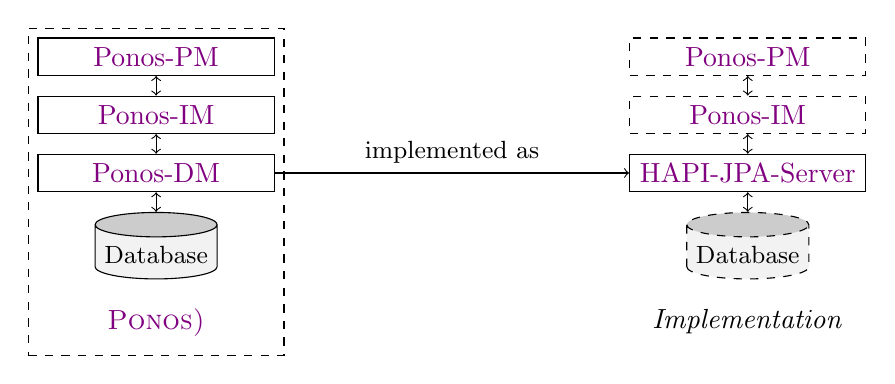
\begin{tikzpicture}[node distance=0.5cm]
            \node[draw,rectangle, minimum width = 3cm](ponospm){\color{Purple}Ponos-PM};
            \node[draw,rectangle, minimum width = 3cm, below=of ponospm, yshift=0.25cm](ponosim){\color{Purple}Ponos-IM};
            \draw[<->](ponospm.south)--(ponosim.north);
            \node[draw,rectangle, minimum width = 3cm, below=of ponosim, yshift=0.25cm](ponosdm){\color{Purple}Ponos-DM};
            \draw[<->](ponosim.south)--(ponosdm.north);
            \node[draw, cylinder, cylinder uses custom fill, cylinder body fill = gray!10, cylinder end fill = gray!40, aspect = 0.2, shape border rotate = 90, , below=of ponosdm, yshift=0.25cm](ponosdb){\small{Database}};
            \draw[<->](ponosdm.south)--(ponosdb.north);
            \node[rectangle, below=of ponosdb,yshift=0.25cm](ponoslabel){\color{Purple}\textsc{Ponos)}};
            \node[draw,rectangle,dashed, fit=(ponospm) (ponoslabel)](ponos){};

            \node[draw,rectangle,dashed, minimum width = 3cm, right=of ponospm, xshift=4cm](ponospm-imp){\color{Purple}Ponos-PM};
            \node[draw,rectangle,dashed, minimum width = 3cm, below=of ponospm-imp, yshift=0.25cm](ponosim-imp){\color{Purple}Ponos-IM};
            \draw[<->](ponospm-imp.south)--(ponosim-imp.north);
            \node[draw,rectangle, minimum width = 3cm, right=of ponosdm, xshift=4cm](hapi-jpa){\color{Purple}HAPI-JPA-Server};
            \draw[<->](ponosim-imp.south)--(hapi-jpa.north);
            \node[draw, dashed, cylinder, cylinder uses custom fill, cylinder body fill = gray!10, cylinder end fill = gray!40, aspect = 0.2, shape border rotate = 90, , below=of hapi-jpa, yshift=0.25cm](database){\small{Database}};
            \draw[<->](hapi-jpa.south)--(database.north);
            \node[rectangle, below=of database,yshift=0.25cm](impl-label){\textit{Implementation}};

            \draw[->](ponosdm.east)--(hapi-jpa.west) node [above, midway]{\small{implemented as}};
        \end{tikzpicture}
	\end{adjustbox}
	\caption{Ponos-DM Implementation Overview}
	\label{fig:ponos-dm-imp}
\end{figure}

The specific details of the \textit{HAPI FHIR JPA Server} subsystem used are detailed in the following library.
\begin{table}[h!]
    \begin{center}
    \small{
    \begin{tabular}{ || l | l  | l | l || }
        \hline
        \textbf{Component Name} & \textbf{Sub-Component Name} & \textbf{Version} & \textbf{Commentary} \\
        \hline
        HAPI JPA Server & HAPI Module &  t.b.d & HAPI Web Archive Release \\
        \hline
         & Wildfly & \wildflyversion & Wildfly Middleware Release\\
        \hline
    \end{tabular}
    }
    \caption{Ponos-DB Postgres Version Details}
    \end{center}
\end{table}

\subsubsection{Ponos-DB}

\paragraph{Overview}

\paragraph{Design (Architecture)}

\subparagraph{Interconnectivity}

\subparagraph{Component(s)}

\subparagraph{Storage}

\paragraph{Implementation}

\subparagraph{Interconnectivity}

\subparagraph{Component(s)}

The \ponosdb subsystem is a \postgres database instance (a separate instances per site) that is coupled to an individual instance of \ponosdm.

\begin{figure}[h!]
	\begin{adjustbox}{max size={0.98\textwidth}{0.9\textheight}, center}
        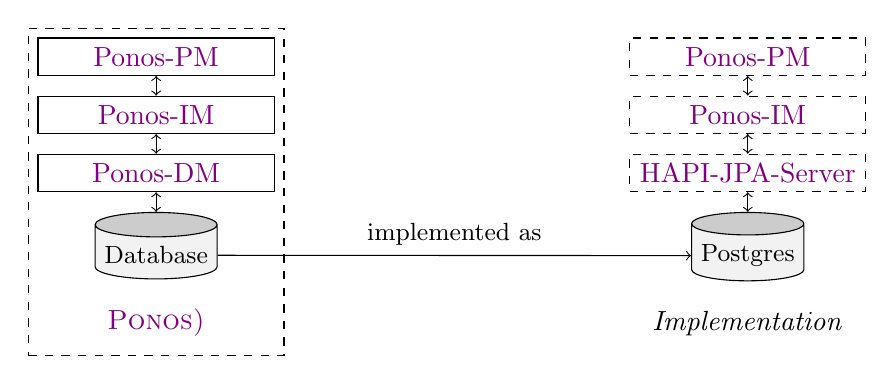
\begin{tikzpicture}[node distance=0.5cm]
            \node[draw,rectangle, minimum width = 3cm](ponospm){\color{Purple}Ponos-PM};
            \node[draw,rectangle, minimum width = 3cm, below=of ponospm, yshift=0.25cm](ponosim){\color{Purple}Ponos-IM};
            \draw[<->](ponospm.south)--(ponosim.north);
            \node[draw,rectangle, minimum width = 3cm, below=of ponosim, yshift=0.25cm](ponosdm){\color{Purple}Ponos-DM};
            \draw[<->](ponosim.south)--(ponosdm.north);
            \node[draw, cylinder, cylinder uses custom fill, cylinder body fill = gray!10, cylinder end fill = gray!40, aspect = 0.2, shape border rotate = 90, , below=of ponosdm, yshift=0.25cm](ponosdb){\small{Database}};
            \draw[<->](ponosdm.south)--(ponosdb.north);
            \node[rectangle, below=of ponosdb,yshift=0.25cm](ponoslabel){\color{Purple}\textsc{Ponos)}};
            \node[draw,rectangle,dashed, fit=(ponospm) (ponoslabel)](ponos){};

            \node[draw,rectangle,dashed, minimum width = 3cm, right=of ponospm, xshift=4cm](ponospm-imp){\color{Purple}Ponos-PM};
            \node[draw,rectangle,dashed, minimum width = 3cm, below=of ponospm-imp, yshift=0.25cm](ponosim-imp){\color{Purple}Ponos-IM};
            \draw[<->](ponospm-imp.south)--(ponosim-imp.north);
            \node[draw,rectangle,dashed, minimum width = 3cm, right=of ponosdm, xshift=4cm](hapi-jpa){\color{Purple}HAPI-JPA-Server};
            \draw[<->](ponosim-imp.south)--(hapi-jpa.north);
            \node[draw, cylinder, cylinder uses custom fill, cylinder body fill = gray!10, cylinder end fill = gray!40, aspect = 0.2, shape border rotate = 90, , below=of hapi-jpa, yshift=0.25cm](database){\small{Postgres}};
            \draw[<->](hapi-jpa.south)--(database.north);
            \node[rectangle, below=of database,yshift=0.25cm](impl-label){\textit{Implementation}};

            \draw[->](ponosdb.east)--(database.west) node [above, midway]{\small{implemented as}};
        \end{tikzpicture}
	\end{adjustbox}
	\caption{Ponos-DB Implementation Overview}
	\label{fig:ponos-db-imp}
\end{figure}

The specific details of the \postgres subsystem used are detailed in the following library.
\begin{table}[h!]
    \begin{center}
    \small{
    \begin{tabular}{ || l | l  | l | l || }
        \hline
        \textbf{Component Name} & \textbf{Sub-Component Name} & \textbf{Version} & \textbf{Commentary} \\
        \hline
        Postgres & Postgres & \postgresversion & Core (executable) Release\\
        \hline
    \end{tabular}
    }
    \caption{Ponos-DB Postgres Version Details}
    \end{center}
\end{table}




\subparagraph{Storage}

The \textit{Storage} for the \ponosdb may be implemented as a single disk (virtual, networked, etc.) or it can be replicated to provide higher levels of assurance. Note that redundancy is typically delivered by \ponosim which replicates content across multiple \ponosdm instances and, thus, across multiple \ponosdb storage services.

\subsection{Hestia.Aduit (Audit Capture / Reporting)}

\subsection{ITOps (Component Monitoring / Reporting)}

\chapter{Middleware Architecture}
\section{Frameworks}
\subsection{Overview}

A key design goal of \textit{DRICATS}, as articulated in its very name, is to support a highly resilient and distributed set of integration, collobaration and tasking services.





\subsubsection{Petasos}

A core enabler of this resilience is the \textit{Petasos} framework - a set of customised modules (software-components) that deliver:
\begin{enumerate}
    \item{\textcolor{OliveGreen}{Reslience via Concurrency:}} Each software process can have multiple instances running concurrently, where-by a single instance is designated as having ``focus'' whilst the others await either successful completion by the ``in-focus'' instance or failure conditions resulting in another instance taking over.
    \item{\textcolor{OliveGreen}{Resilience via Asynchronous Monitoring:}} Each ``activity'' is monitored - to detect failure states (e.g. exceptions, inifinite-loops, etc.) with resulting termination of the failured process ``thread'' and execution to an alternate instance.
    \item{\textcolor{OliveGreen}{Resilience via Recovery:}} Each ``activity'' is, as well as having multiple instances of itself ready to be processed, also ``archived'' into (one or more) persistent stores as a mechanism to recover from catastrophic system failure.
 \end{enumerate}
\subsubsection{Task}

\subsection{Component Architypes}
\subsubsection{ProcessingPlants}
\subsubsection{Workshops}

\subsubsection{WorkUnitProcessors}

\paragraph{Overview}

\begin{figure}[h!]
	\begin{adjustbox}{max size={0.98\textwidth}{0.9\textheight}, center}
		\includegraphics[]{diagrams/Petasos-WUP.png}
	\end{adjustbox}
	\caption{Work Unit Processor / Petasos - Logical Architecture}
\end{figure}



\paragraph{\textsc{Petasos} Local Task Distribution Services}

\paragraph{\textsc{Petasos} Local Task Monitoring Services}

\paragraph{\textsc{Petasos} Local Task Reporting Services}

\paragraph{\textsc{Petasos} Distributed Messaging Services}

\subsubsection{Endpoint}

\subsection{FHIR-DataGrid}
\subsubsection{Cache}
\subsubsection{Persistence-Adapter}

\subsection{FHIR-Datastore}
\subsubsection{FHIR.DM: HAPI\texttrademark Java Persistence API Server}
\subsubsection{FHIR.DB: Postgres DBaaS}

\section{Middleware Platforms}
\subsection{Apache\textsuperscript{\textregistered} Camel\texttrademark}
\subsection{Wildfly\texttrademark}
\subsection{Postgres}
\subsection{NodeJS}
\subsection{Infinispan\textsuperscript{\textregistered}}
\subsection{JGroups\texttrademark}
\subsection{JakartaEE\texttrademark}

\part{Technology Architecture}
\chapter{Data Architecture}

\chapter{Logical Architecture}

\chapter{Physical Architecture}

\appendix

\chapter{Petasos}
\label{epic:petasos}
\section{Overview}
    \petasos is the core capability delivery framework of the \dricats system and is responsible, within each application, for ensuring effective \textit{function delivery} (i.e. the throughput, reliability and scalability) and \textit{function assurance} (i.e. recovery, reporting and metrics) of system behaviour.

    \petasos is comprised of several building blocks - some which operate within each individual application \textit{POD}, others which span all \textit{PODs} delivering a specific application (\textit{service}) whilst others require peer functionality within \textit{enabler} subsystems (such as \textbf{ITOps}, \textbf{Ladon} and \textbf{Ponos}).

    This \textit{Appendix} details the functional, conceptual, logical and deployment architecture of the \petasos framework - as used within the various subsystems comprising a \dricats deployment.

    With the exception of the \textbf{Petasos-Interzone-Repeater}, a \textbf{JGroups} based reliable messaging and \textit{Remote Method Invocation} framework, \petasos does not have a stand-alone component. It is implemented and delivered as enablers within the various other subsytems. It, in turn, is enabled by the \textbf{Ladon}, \textbf{Hestia.Audit}, \textbf{ITOps} and \textbf{Ponos} subsystems.
\section{Functional Architecture}
\subsection{Overview}
    \begin{figure}[h!]
        \begin{adjustbox}{max size={0.98\textwidth}{0.9\textheight}, center}
            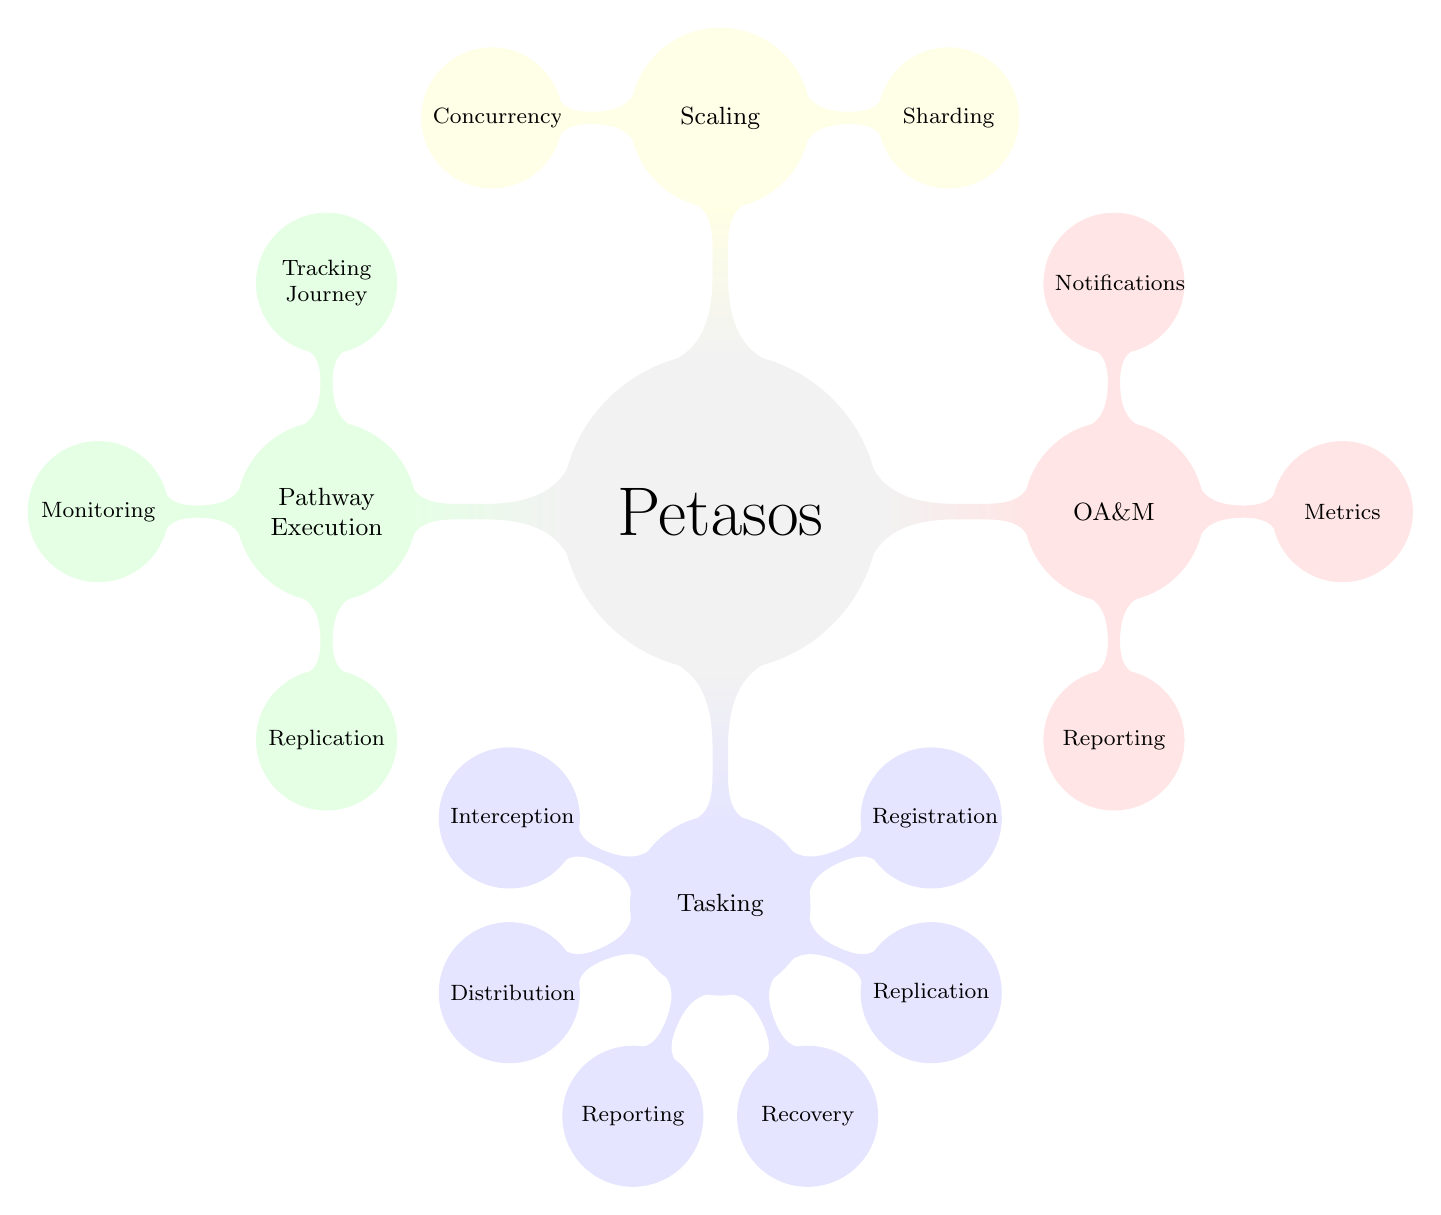
\begin{tikzpicture}
            \path[mindmap,concept color=gray!10,text=black]
                node[concept] {\Huge{Petasos}}[clockwise from=0, level 1 concept/.append style={sibling angle=90}]
                child[concept color=red!10, text=black] { node[concept] {OA\&M}[clockwise from=90, , level 2 concept/.append style={sibling angle=90}]
                    child { node[concept] {Notifications} }
                    child { node[concept] {Metrics} }
                    child { node[concept] {Reporting} }}
                child[concept color=blue!10] { node[concept] {Tasking} [clockwise from=22.5, level 2 concept/.append style={sibling angle=45}]
                    child { node[concept] {Registration} }
                    child { node[concept] {Replication} }
                    child { node[concept] {Recovery} }
                    child { node[concept] {Reporting} }
                    child { node[concept] {Distribution} }
                    child { node[concept] {Interception} }}
                child[concept color=green!10] { node[concept] {Pathway\\Execution} [clockwise from=-90, level 2 concept/.append style={sibling angle=90}]
                    child { node[concept] {Replication} }
                    child { node[concept] {Monitoring} }
                    child { node[concept] {Tracking\\Journey} }}
                child[concept color=yellow!10] { node[concept] {Scaling} [clockwise from=-180, level 2 concept/.append style={sibling angle=180}]
                    child { node[concept] {Concurrency} }
                    child { node[concept] {Sharding} }};
            \end{tikzpicture}
        \end{adjustbox}
        \caption{Petasos - Functional Architecture}
        \label{fig:functional-architecture-petasos-overview}
    \end{figure}

    The functional architecture, as illustrated in the figure below (see Figure \ref{fig:functional-architecture-petasos-overview}), encapsulates the following enabling functions and services:
    \begin{itemize}
        \item \textit{Operations, Administration \& Maintenance (OA\&M)}: Whilst the whole of \petasos may be considered an OA\&M function, it is useful to distinguish the actual OA\&M functions separately. OA\&M functions are, as their name suggest, the functions of the system that are used to monitor and report the effective (or otherwise) operation of the system (subsystem). \petasos includes the following general OA\&M functions:
        \begin{itemize}
            \item \textit{Notifications:} Asynchronous events/updates, distributed via various communication channels (and user interfaces) that communicate any ``abnormal'' or ``note-worthy'' event within the system.
            \item \textit{Metrics:} Worthwhile statics and parameters that detail the present-state (and historical) view of the subsystem.
            \item \textit{Reporting:} System (subsytem) Events/ and checkpoints of ``note'', reported using a well-defined framework pertaining to the activity in question. \petasos uses two forms of reporting, a FHIR::AuditEvent based reporting log and a FHIR::Task centric activity database. The content in both is visible via various user interfaces.
        \end{itemize}
        \item \textit{Pathway Execution:} At its heart, the \petasos framework implements key functions to ensure the effective \textbf{processing} and \textbf{completion} of \textbf{Tasks}. Within the context of a \textit{Message Integration Engine}, this \textit{``task completion''} is manifested as an assurance that messages \textbf{received by it} are captured, processed and, if appropriate, \textbf{forwarded by it} - if appropriate. The \textit{Pathway Execution} functions include:
        \begin{itemize}
            \item \textit{Replication:} Irrespective of the activity being undertaken (i.e. message processing, task processing, etc.) - all activities are encapsulated within an \textit{ActionableTask} as something that ``needs to be fulfilled''. These \textit{ActionableTask's} are replicated within an application specific cache to all other ``instances'' implementing the same application function. This replication forms a part of a \textbf{localised} (to the application instance type) resilience and recovery framework - whereby all instances of the application are capable of executing (``fulfilling'') the \textit{ActionalTask} if the origin executor fails or times-out.
            \item \textit{Monitoring:} At a local level (i.e. within the context of the application (subsystem instance), ``watchdog'' functionality monitors and takes corrective action for any \textit{ActionableTasks} that have failed to be completed. This \textit{Monitoring} functionality also tightly couples with the \textit{OA\&M} functions to provide notifications and alerts as to asymptomatic behaviours.
            \item \textit{Task Hand-Off/Journey:} Within the local environment (of a single ``application'' or ``POD''), ensuring that the completion of one \textit{ActionableTask} is processed, audited and a successor kickstarted (with suitable monitoring of successful launch) is also managed.
        \end{itemize}
        \item \textit{Scaling:}
        \begin{itemize}
            \item \textit{Concurrency:} Executing multiple instances doing the ``same'' thing allows for increased throughput and rapid recovery in failure conditions.
            \item \textit{Sharding:} Splitting up the processing, based on content, function, origin or target means that the framework can scale in multiple ways - all via configuration rather than code changes.
        \end{itemize}
        \item \textit{Tasking:}
        \begin{itemize}
            \item \textit{Registration:} The \textit{registration} of \textit{tasks} (and other activities) to a \textit{logically centralised, physically replicated/distributed} framework (i.e. the \ponos subsystem) provides a very high level of resilience - beyond single application/service boundaries. The capability goes beyond the \textit{Replication} function to provide a \textit{logically centralised} recovery, suspend/resume and monitoring point.
            \item \textit{Replication:} Each \textit{application} delivering a particular \textit{service} within the \dricats framework (and built on the \petasos framework) makes use of a ``shared cache'' with other instances of the same \textit{application} type. This cache ensures that the content of an \textit{ActionableTask} being implemented is replicated across ALL instances in real-time. Failure of a single \textit{POD} in which an \textit{application} instance is executing results in no loss of information - beyond in-flight computations. The \textit{PathwayExecution::Replication} function identified above ensures that there are multiple instances of the \textit{application} available to ``pick-up'' the processing under failure conditions.
            \item \textit{Recovery:} The \textit{Recovery} framework for \textit{tasks} comprises three (3) tiers of capability:
            \begin{itemize}
                \item \textit{Local Cache Availability:} Firstly, the actual \textit{FulfillmentTask\footnote{The \textit{FulfillmentTask} is the encapsulation of task state for the actual implementation/fulfillment of the activity pertaining to the \textit{ActionableTask}.}} being undertaken within application has a snapshot stored in a local cache for recovery/retry purposes (\textit{PathwayExecution::Tracking/Journey, PathwayExecution::Monitoring}).
                \item \textit{Shared Cache Availability:} The base \textit{ActionableTask} is persisteted across of application instant types for the purposes of recovery and re-try via another application instant - if this instant fails processing the task more than a configurable number or times or fails/terminates for some reason.
                \item \textit{Task Repository:} The base \textit{ActionableTask} is registered  with a centralised repository (see \ref{feature:petasos.tasking.registration}) for the purposes of ``global'' monitoring, suspend/resume and recovery activities.
            \end{itemize}
            \item \textit{Reporting:}
            \item \textit{Distribution:}
            \item \textit{Interception:}
        \end{itemize}
    \end{itemize}

\subsection{Operations, Administration \& Maintenance (OA\&M)}
\label{feature:petasos.oam}
\subsubsection{Notifications}
\label{feature:petasos.oam.notification}

\subsubsection{Metrics}
\label{feature:petasos.oam.metrics}

\subsubsection{Reporting}
\label{feature:petasos.oam.reporting}

\subsection{Scaling}
\label{feature:petasos.scaling}
\subsubsection{Concurrency}
\label{feature:petasos.scaling.concurrency}

\subsubsection{Sharding}
\label{feature:petasos.scaling.sharding}

\subsection{Pathway Execution}
\label{feature:petasos.pathway}

\subsubsection{Replication}
\label{feature:petasos.pathway.replication}
\subsubsection{Monitoring}
\label{feature:petasos.pathway.monitoring}
\subsubsection{Task Hand-Off / Journey}
\label{feature:petasos.pathway.handoff}

\subsection{Tasking}
\label{feature:petasos.tasking}
\subsubsection{Registration}
\label{feature:petasos.tasking.registration}
\subsubsection{Replication}
\subsubsection{Recovery}
\subsubsection{Reporting}
\subsubsection{Distribution}
\subsubsection{Interception}

\section{Conceptual Architecture}
\section{Logical Architecture}
\section{Deployment Architecture}

\chapter{Ponos}
\section{Overview}
\subsection{Functional Overview}

\begin{figure}[h!]
\begin{adjustbox}{max size={0.98\textwidth}{0.9\textheight}, center}
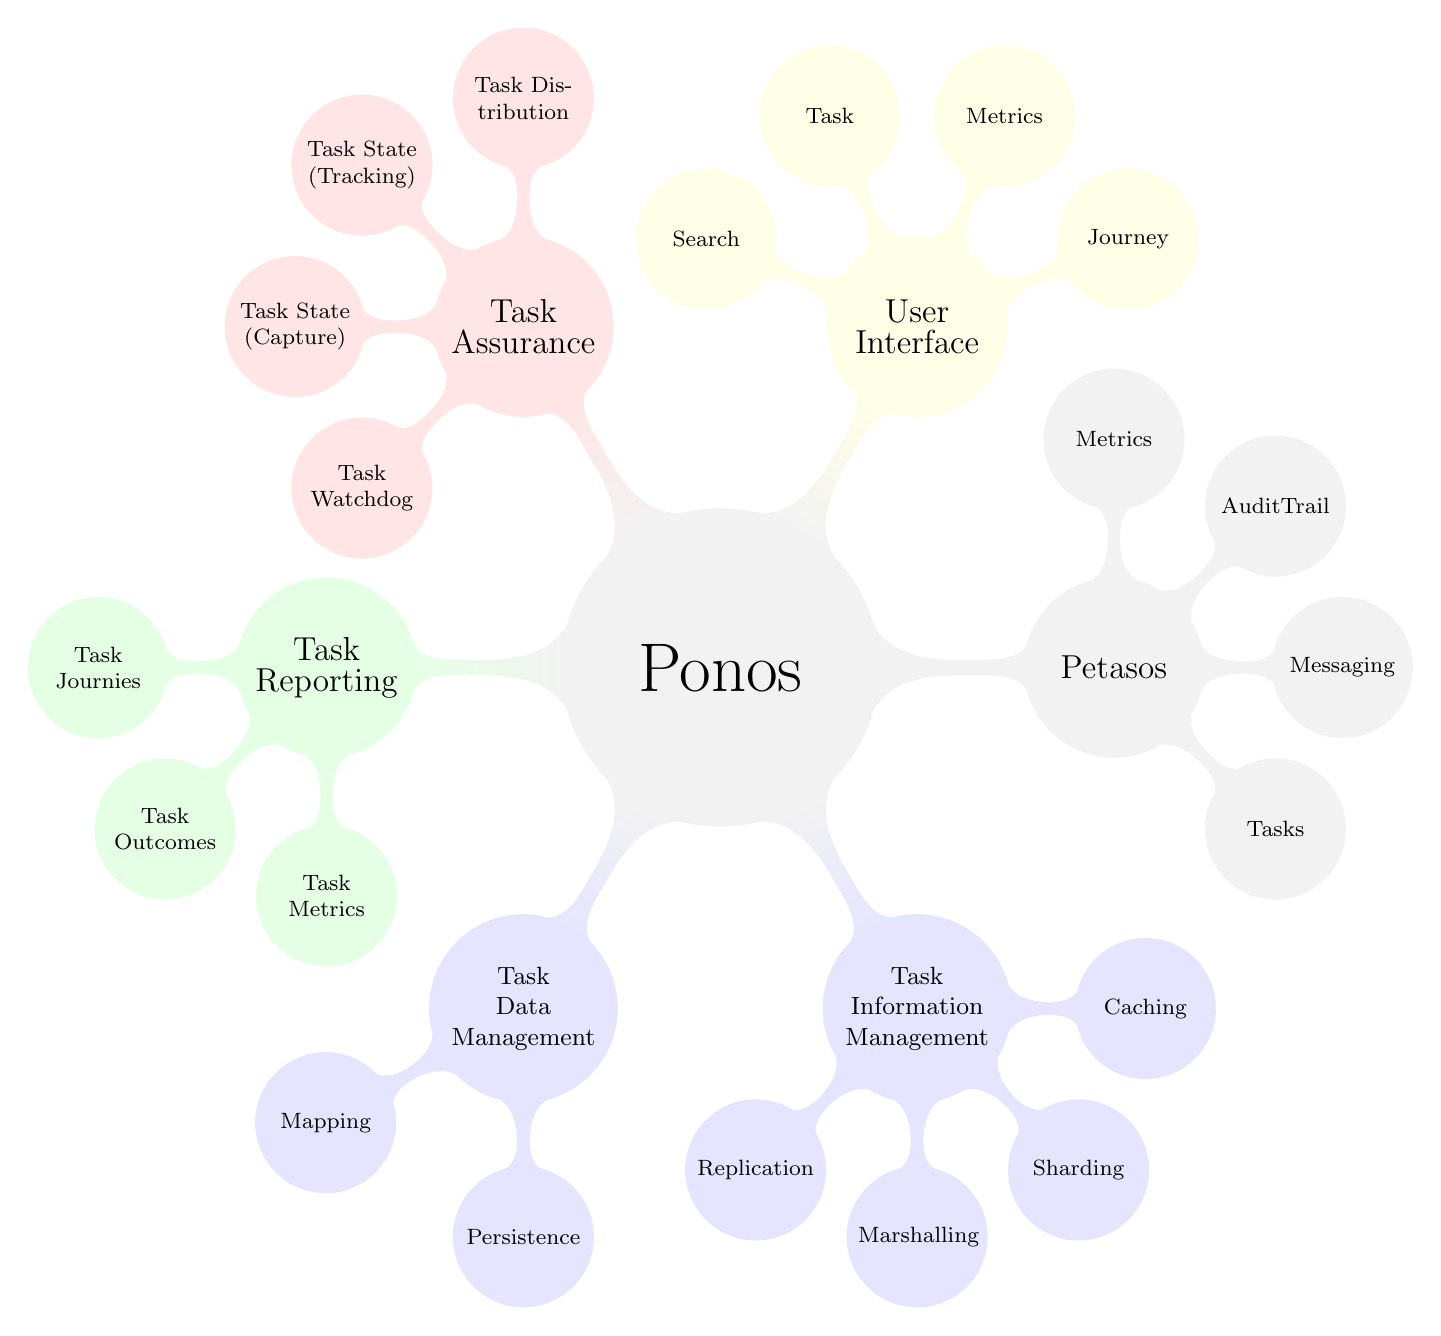
\begin{tikzpicture}
\path[mindmap,concept color=gray!10,text=black]
    node[concept] {\Huge{Ponos}}[clockwise from=0]
    child[concept color=gray!10, text=black] { node[concept] {\large{Petasos}}[clockwise from=90, level 2 concept/.append style={sibling angle=45}]
        child { node[concept] {Metrics} }
        child { node[concept] {AuditTrail} }
        child { node[concept] {Messaging} }
        child { node[concept] {Tasks} }}
    child[concept color=blue!10] { node[concept] {Task\\ Information\\ Management} [clockwise from=0,level 2 concept/.append style={sibling angle=45}]
        child { node[concept] {Caching} }
        child { node[concept] {Sharding} }
        child { node[concept] {Marshalling} }
        child { node[concept] {Replication} }}
    child[concept color=blue!10] { node[concept] {Task\\ Data\\ Management} [clockwise from=-90]
        child { node[concept] {Persistence} }
        child { node[concept] {Mapping} }}
    child[concept color=green!10] { node[concept] {\large{Task Reporting}} [clockwise from=-90, level 2 concept/.append style={sibling angle=45}]
        child { node[concept] {Task Metrics} }
        child { node[concept] {Task Outcomes} }
        child { node[concept] {Task Journies} }}
    child[concept color=red!10, text=black] { node[concept] {\large{Task Assurance}}[clockwise from=-135, level 2 concept/.append style={sibling angle=45}]
        child { node[concept] {Task Watchdog} }
        child { node[concept] {Task State (Capture)} }
        child { node[concept] {Task State (Tracking)} }
        child { node[concept] {Task Distribution} }}
    child[concept color=yellow!10] { node[concept] {\large{User Interface}} [clockwise from=-202.5, level 2 concept/.append style={sibling angle=45}]
        child { node[concept] {Search} }
        child { node[concept] {Task} }
        child { node[concept] {Metrics} }
        child { node[concept] {Journey} }};
\end{tikzpicture}
\end{adjustbox}
\end{figure}

\section{Conceptual Architecture}
\subsection{Subsystem Breakdown}

The following diagram illustrates the subsystem breakdown of the \ponos subsystem.

\begin{figure}[h!]
\begin{adjustbox}{max size={0.95\textwidth}{0.9\textheight}, center}
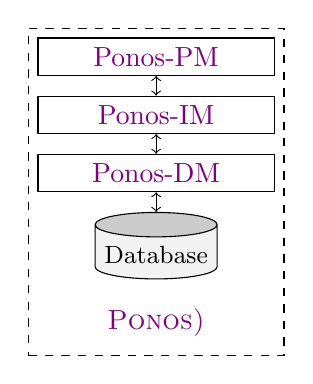
\begin{tikzpicture}[node distance=0.5cm]
    \node[draw,rectangle, minimum width = 3cm](ponospm){\color{Purple}Ponos-PM};
    \node[draw,rectangle, minimum width = 3cm, below=of ponospm, yshift=0.25cm](ponosim){\color{Purple}Ponos-IM};
    \draw[<->](ponospm.south)--(ponosim.north);
    \node[draw,rectangle, minimum width = 3cm, below=of ponosim, yshift=0.25cm](ponosdm){\color{Purple}Ponos-DM};
    \draw[<->](ponosim.south)--(ponosdm.north);
    \node[draw, cylinder, cylinder uses custom fill, cylinder body fill = gray!10, cylinder end fill = gray!40, aspect = 0.2, shape border rotate = 90, , below=of ponosdm, yshift=0.25cm](ponosdb){\small{Database}};
    \draw[<->](ponosdm.south)--(ponosdb.north);
    \node[rectangle, below=of ponosdb,yshift=0.25cm](ponoslabel){\color{Purple}\textsc{Ponos)}};
    \node[draw,rectangle,dashed, fit=(ponospm) (ponoslabel)](ponos){};
\end{tikzpicture}
\end{adjustbox}
\caption{Ponos Subsystem Overview}
\label{fig:ponos-subsystem-overview}
\end{figure}

The \ponos subsystem, like many other \dricats subsystems, is typically implemented as four discrete applications - each executing within their own container (set) within a \textit{Kubernetes} environment. These applications are:
\begin{itemize}[noitemsep]
 \item a presentation management application;
 \item an information management / business logic application;
 \item a data management framework / application; and
 \item a data persistence framework / application.
\end{itemize}

It is also worthwhile noting that \ponos implments data resilience via replication at the application-level - within the ``information management'' tier. Any resilience delivered by the infrastructure (technology) layer, the peristence framework/tier, the data management framework/tier provides a \textbf{secondary} level of data/information resilience.

\section{Logical Architectire}
\section{Deployment Architecture}

\chapter{Hestia.Audit}
\section{Overview}
\section{Conceptual Architecture}
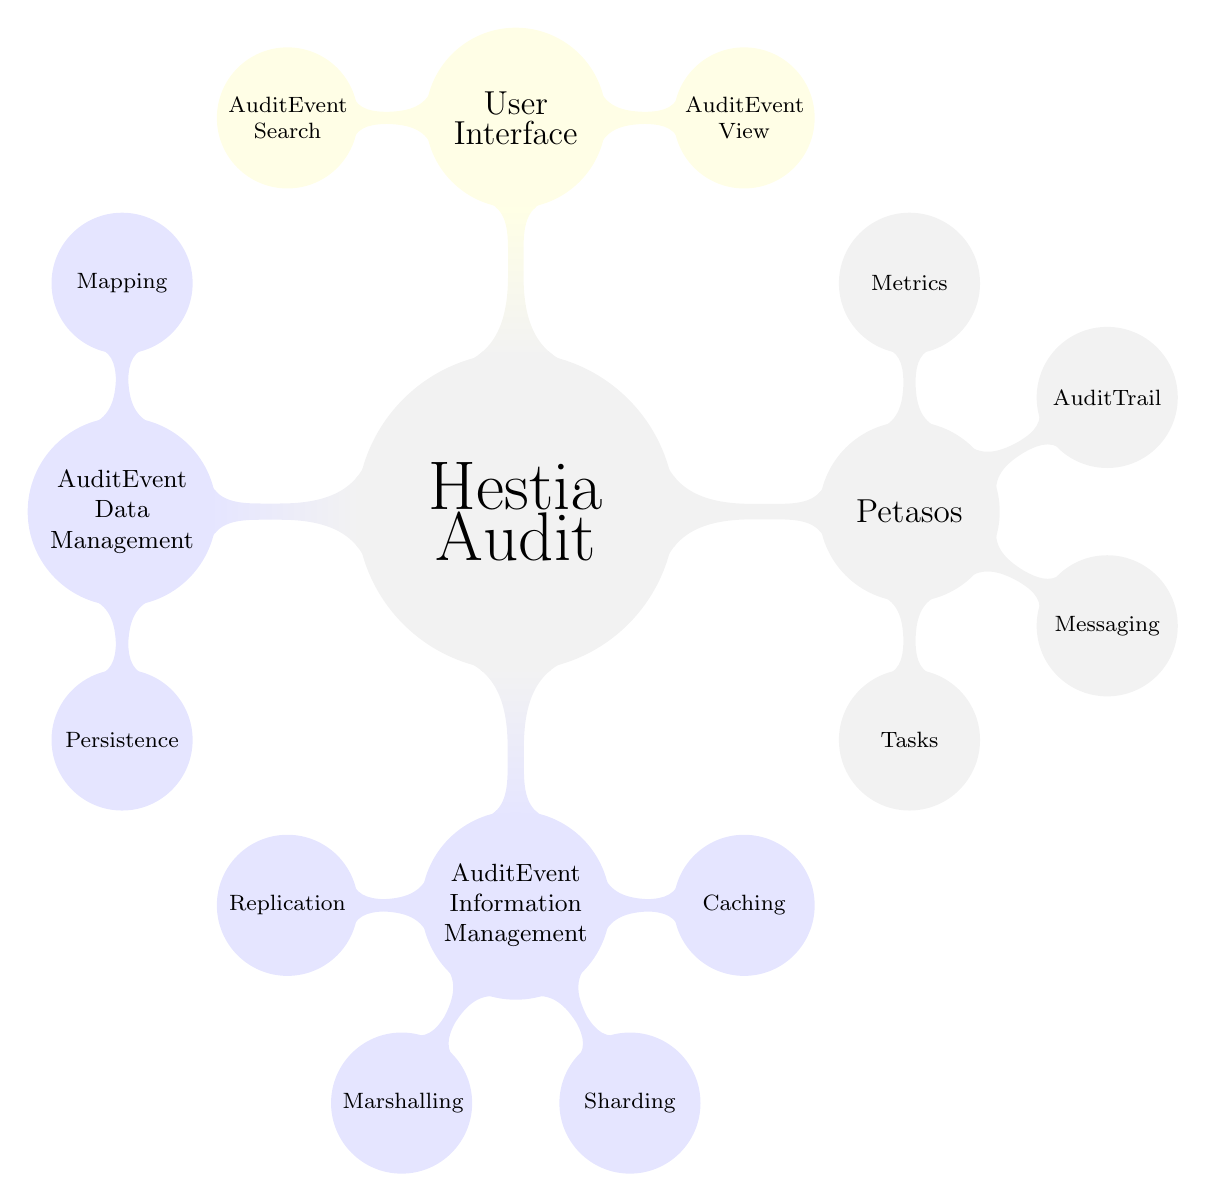
\begin{tikzpicture}
\path[mindmap,concept color=gray!10,text=black]
    node[concept] {\Huge{Hestia\\Audit}}[clockwise from=0, level 1 concept/.append style={sibling angle=90}]
    child[concept color=gray!10, text=black] { node[concept] {\large{Petasos}}[clockwise from=90]
        child { node[concept] {Metrics} }
        child { node[concept] {AuditTrail} }
        child { node[concept] {Messaging} }
        child { node[concept] {Tasks} }}
    child[concept color=blue!10] { node[concept] {AuditEvent\\ Information\\ Management} [clockwise from=0]
        child { node[concept] {Caching} }
        child { node[concept] {Sharding} }
        child { node[concept] {Marshalling} }
        child { node[concept] {Replication} }}
    child[concept color=blue!10] { node[concept] {AuditEvent\\ Data\\ Management} [clockwise from=-90, level 2 concept/.append style={sibling angle=180}]
        child { node[concept] {Persistence} }
        child { node[concept] {Mapping} }}
    child[concept color=yellow!10] { node[concept] {\large{User Interface}} [clockwise from=-180, level 2 concept/.append style={sibling angle=180}]
        child { node[concept] {AuditEvent Search} }
        child { node[concept] {AuditEvent View} }};
\end{tikzpicture}
\section{Logical Architectire}
\section{Deployment Architecture}

\chapter{Hestia.DAM}
\section{Overview}
\section{Conceptual Architecture}
\section{Logical Architectire}
\section{Deployment Architecture}

\chapter{Ladon}
\section{Overview}
\section{Conceptual Architecture}
\section{Logical Architectire}
\section{Deployment Architecture}

\chapter{Navigator}
\section{Overview}
\section{Conceptual Architecture}
\section{Logical Architectire}
\section{Deployment Architecture}

\chapter{MITaF-PAS}
\section{Overview}
\section{Conceptual Architecture}
\section{Logical Architectire}
\section{Deployment Architecture}

\chapter{MITaF-SMTP}
\section{Overview}
\section{Conceptual Architecture}
\section{Logical Architectire}
\section{Deployment Architecture}

\chapter{MITaF-TAP}
\section{Overview}
\section{Conceptual Architecture}
\section{Logical Architectire}
\section{Deployment Architecture}

\chapter{MITaF-HL7v2}
\section{Overview}
\section{Conceptual Architecture}
\section{Logical Architectire}
\section{Deployment Architecture}

\chapter{FHIRBreak-Files}
\section{Overview}
\section{Business Services}
\begin{figure}[h!]
\begin{adjustbox}{max size={0.95\textwidth}{0.9\textheight}, center}
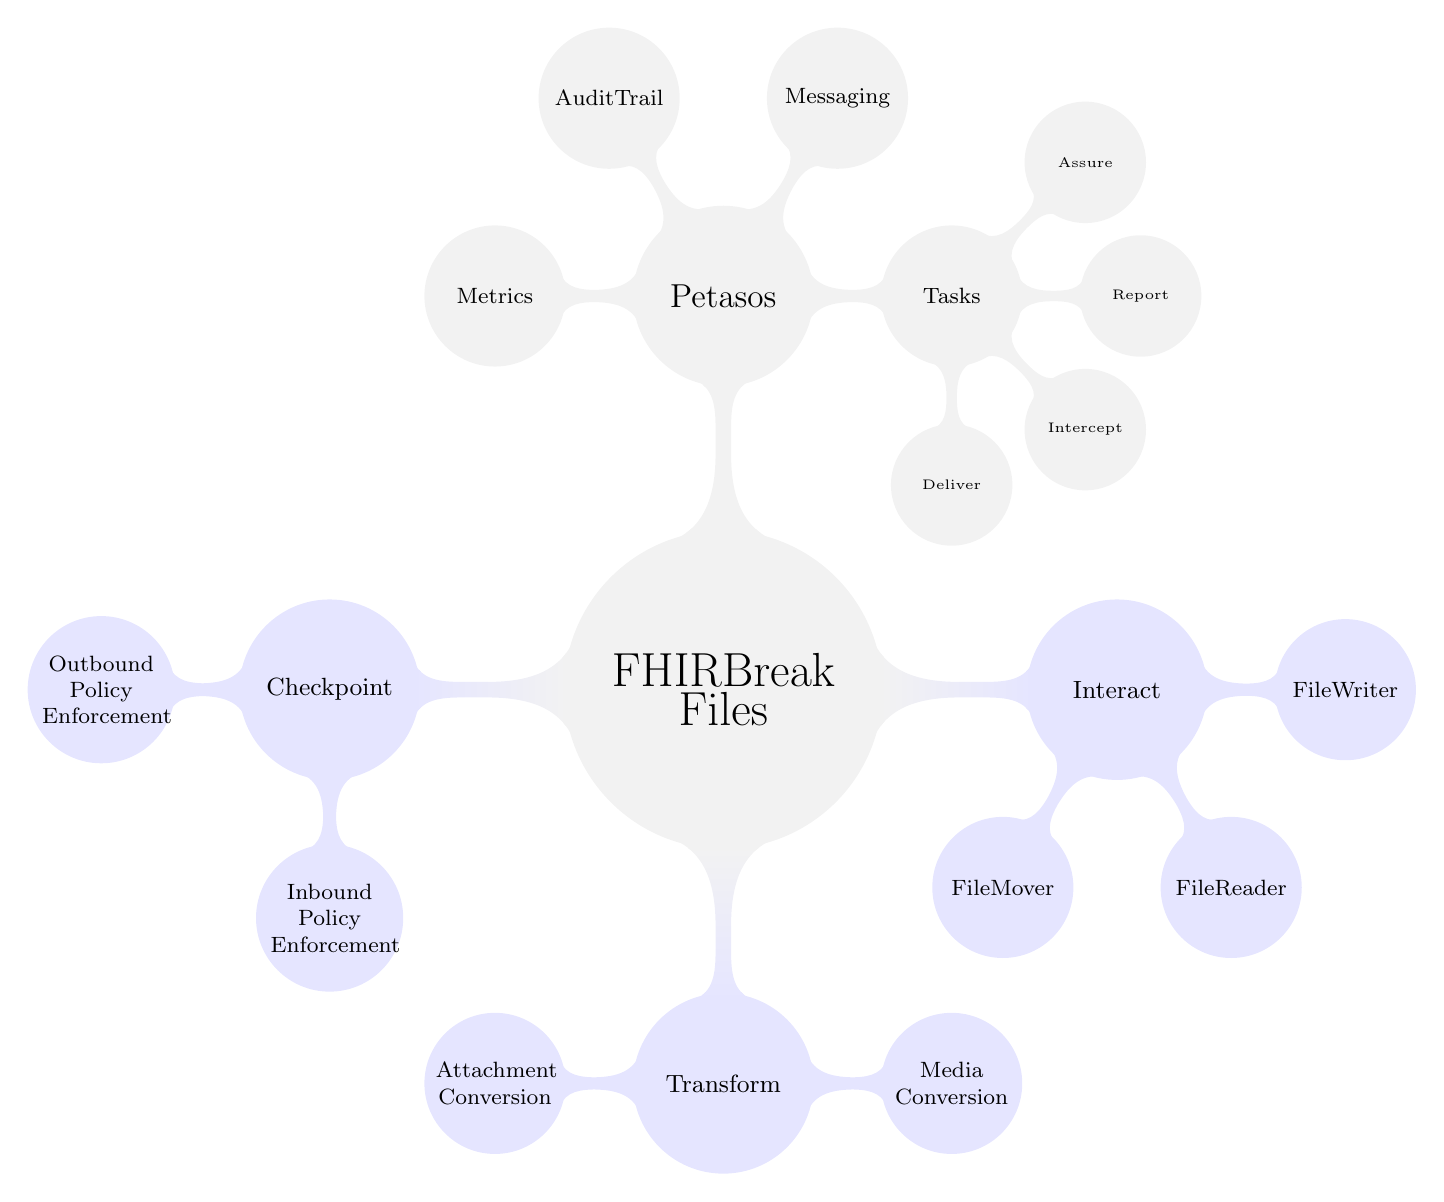
\begin{tikzpicture}
\path[mindmap,concept color=gray!10,text=black]
    node[concept] {\LARGE{FHIRBreak\\Files}}[clockwise from=90, level 1 concept/.append style={sibling angle=90}]
    child[concept color=gray!10, text=black] { node[concept] {\large{Petasos}}[clockwise from=180]
        child { node[concept] {Metrics} }
        child { node[concept] {AuditTrail} }
        child { node[concept] {Messaging} }
        child[concept] { 
            node[concept] {Tasks} [clockwise from=45, level 3 concept/.append style={sibling angle=45}]
                child { node[concept, minimum size=1.5cm] {Assure} }
                child { node[concept, minimum size=1.5cm] {Report} }
                child { node[concept, minimum size=1.5cm] {Intercept} }
                child { node[concept, minimum size=1.5cm] {Deliver} 
            }
        }
    }
    child[concept color=blue!10] { 
        node[concept] {Interact} [clockwise from=0]
            child { node[concept] {FileWriter} }
            child { node[concept] {FileReader} }
            child { node[concept] {FileMover} }
    }
    child[concept color=blue!10] { node[concept] {Transform} [clockwise from=0,level 2 concept/.append style={sibling angle=180}]
        child { node[concept] {Media\\Conversion} }
        child { node[concept] {Attachment\\Conversion} }}
    child[concept color=blue!10] { node[concept] {Checkpoint} [clockwise from=-90, level 2 concept/.append style={sibling angle=90}]
        child { node[concept] {Inbound Policy \\ Enforcement} }
        child { node[concept] {Outbound Policy \\ Enforcement} }};
\end{tikzpicture}
\end{adjustbox}
\caption{FHIRBreak-Files Function Map}
\label{fig:ponos-subsystem-overview}
\end{figure}
\section{Conceptual Architecture}
\section{Logical Architectire}
\section{Deployment Architecture}

\chapter{FHIRBreak-SMS}
\section{Overview}
\section{Conceptual Architecture}
\section{Logical Architectire}
\section{Deployment Architecture}

\chapter{FHIRBreak-EDW}
\section{Overview}
\section{Conceptual Architecture}
\section{Logical Architectire}
\section{Deployment Architecture}

\chapter{FHIRBreak-PAS}
\section{Overview}
\section{Conceptual Architecture}
\section{Logical Architectire}
\section{Deployment Architecture}

\chapter{ITOps}
\section{Overview}
\section{Conceptual Architecture}
\section{Logical Architectire}
\section{Deployment Architecture}
\end{document}

